
\documentclass{article}

\usepackage{fancyhdr} % Required for custom headers
\usepackage{lastpage} % Required to determine the last page for the footer
\usepackage{extramarks} % Required for headers and footers
\usepackage[usenames,dvipsnames]{color} % Required for custom colors
\usepackage{graphicx} % Required to insert images
\usepackage{listings} % Required for insertion of code
\usepackage{courier} % Required for the courier font
\usepackage{lipsum} % Used for inserting dummy 'Lorem ipsum' text into the template
\usepackage{caption}
\usepackage{subcaption}
\usepackage{mathtools}
\usepackage{amsmath}
\usepackage{esint}
\usepackage{physics}
\usepackage{color}
\usepackage{listings}
\usepackage{pythonhighlight}

\graphicspath{ {../../../datasets/images/chapter_02/} }

% Margins
\topmargin=-0.45in
\evensidemargin=0in
\oddsidemargin=0in
\textwidth=6.5in
\textheight=9.0in
\headsep=0.25in

\linespread{1.1} % Line spacing

% Set up the header and footer
\pagestyle{fancy}
\lhead{\hmwkAuthorName} % Top left header
\chead{\hmwkClass\ (\hmwkClassInstructor\ \hmwkClassTime): \hmwkTitle} % Top center head
\rhead{\firstxmark} % Top right header
\lfoot{\lastxmark} % Bottom left footer
\cfoot{} % Bottom center footer
\rfoot{Page\ \thepage\ of\ \protect\pageref{LastPage}} % Bottom right footer
\renewcommand\headrulewidth{0.4pt} % Size of the header rule
\renewcommand\footrulewidth{0.4pt} % Size of the footer rule

\setlength\parindent{0pt} % Removes all indentation from paragraphs

%----------------------------------------------------------------------------------------
%	CODE INCLUSION CONFIGURATION
%----------------------------------------------------------------------------------------

\definecolor{MyDarkGreen}{rgb}{0.0,0.4,0.0} 
\lstloadlanguages{Matlab}
\lstset{language=Matlab,
        frame=single,
        basicstyle=\small\ttfamily,
        keywordstyle=[1]\color{Blue}\bf,
        keywordstyle=[2]\color{Purple},
        keywordstyle=[3]\color{Blue}\underbar,
        identifierstyle=,
        commentstyle=\usefont{T1}{pcr}{m}{sl}\color{MyDarkGreen}\small, 
        stringstyle=\color{Purple},
        showstringspaces=false,
        tabsize=5, 
        morekeywords={rand},
        morekeywords=[2]{on, off, interp},
        morekeywords=[3]{test},
        morecomment=[l][\color{Blue}]{...},
        numbers=left,
        firstnumber=1,
        numberstyle=\tiny\color{Blue},
        stepnumber=5
}

% Creates a new command to include a perl script, the first parameter is the filename of the script (without .pl), the second parameter is the caption
\newcommand{\matlabscript}[2]{
\begin{itemize}
\item[]\lstinputlisting[caption=#2,label=#1]{#1.m}
\end{itemize}
}

%----------------------------------------------------------------------------------------
%	DOCUMENT STRUCTURE COMMANDS
%	Skip this unless you know what you're doing
%----------------------------------------------------------------------------------------

% Header and footer for when a page split occurs within a problem environment
\newcommand{\enterProblemHeader}[1]{
\nobreak\extramarks{#1}{#1 continued on next page\ldots}\nobreak
\nobreak\extramarks{#1 (continued)}{#1 continued on next page\ldots}\nobreak
}

% Header and footer for when a page split occurs between problem environments
\newcommand{\exitProblemHeader}[1]{
\nobreak\extramarks{#1 (continued)}{#1 continued on next page\ldots}\nobreak
\nobreak\extramarks{#1}{}\nobreak
}

\setcounter{secnumdepth}{0} % Removes default section numbers
\newcounter{homeworkProblemCounter} % Creates a counter to keep track of the number of problems

\newcommand{\homeworkProblemName}{}
\newenvironment{homeworkProblem}[1][Problem \arabic{homeworkProblemCounter}]{ % Makes a new environment called homeworkProblem which takes 1 argument (custom name) but the default is "Problem #"
\stepcounter{homeworkProblemCounter} % Increase counter for number of problems
\renewcommand{\homeworkProblemName}{#1} % Assign \homeworkProblemName the name of the problem
\section{\homeworkProblemName} % Make a section in the document with the custom problem count
\enterProblemHeader{\homeworkProblemName} % Header and footer within the environment
}{
\exitProblemHeader{\homeworkProblemName} % Header and footer after the environment
}

\newcommand{\problemAnswer}[1]{ % Defines the problem answer command with the content as the only argument
\noindent\framebox[\columnwidth][c]{\begin{minipage}{0.98\columnwidth}#1\end{minipage}} % Makes the box around the problem answer and puts the content inside
}

\newcommand{\homeworkSectionName}{}
\newenvironment{homeworkSection}[1]{ % New environment for sections within homework problems, takes 1 argument - the name of the section
\renewcommand{\homeworkSectionName}{#1} % Assign \homeworkSectionName to the name of the section from the environment argument
\subsection{\homeworkSectionName} % Make a subsection with the custom name of the subsection
\enterProblemHeader{\homeworkProblemName\ [\homeworkSectionName]} % Header and footer within the environment
}{
\enterProblemHeader{\homeworkProblemName} % Header and footer after the environment
}

%----------------------------------------------------------------------------------------
%	NAME AND CLASS SECTION
%----------------------------------------------------------------------------------------

\newcommand{\hmwkTitle}{Assignment\ \#2}
\newcommand{\hmwkDueDate}{Wednesday,\ September\ 27,\ 2017}
\newcommand{\hmwkClass}{3-D\ DIVISION} % Course/class
\newcommand{\hmwkClassTime}{15:00pm} % Class/lecture time
\newcommand{\hmwkClassInstructor}{leecw} % Teacher/lecturer
\newcommand{\hmwkAuthorName}{Tien Anh Nguyen} % Your name

%----------------------------------------------------------------------------------------
%	TITLE PAGE
%----------------------------------------------------------------------------------------

\title{
\vspace{2in}
\textmd{\textbf{\hmwkClass:\ \hmwkTitle}}\\
\normalsize\vspace{0.1in}\small{Due\ on\ \hmwkDueDate}\\
\vspace{0.1in}\large{\textit{\hmwkClassInstructor\ \hmwkClassTime}}
\vspace{3in}
}

\author{\textbf{\hmwkAuthorName}}
\date{} % Insert date here if you want it to appear below your name

%----------------------------------------------------------------------------------------

\begin{document}

\maketitle

%----------------------------------------------------------------------------------------
%	TABLE OF CONTENTS
%----------------------------------------------------------------------------------------

%\setcounter{tocdepth}{1} % Uncomment this line if you don't want subsections listed in the ToC

\newpage
\tableofcontents
\newpage

%----------------------------------------------------------------------------------------
%	PROBLEM 1
%----------------------------------------------------------------------------------------

% To have just one problem per page, simply put a \clearpage after each problem

\begin{homeworkProblem}
\maketitle
\subsection{Radial Distortion}
    \begin{equation}
        \begin{aligned}
            x_{corrected} = x(1 + k_1r^2 + k_2r^4 + k_3r^6)\\
            y_{corrected} = y(1 + k_1r^2 + k_2r^4 + k_3r^6)
        \end{aligned}
    \end{equation}

The point (x, y) of the input a image will be convert to point $(x_{corrected}, y_{corrected})$.
The tangential distortion problem ouccurs, because the lenses cannot perfectly parallel the imaging plane.
    \begin{equation}
        \begin{aligned}
            x_{corrected} = x + [2p_1xy + p_2(r^2 + 2x^2)]\\
            y_{corrected} = y + [p_1(r_2 + 2y_2) + 2p_2xy]
        \end{aligned}
    \end{equation}

So we have totally 5 parameters:

    \begin{equation}
        \begin{aligned}
            Distortion_{coefficients} = (k_1\ k_2\ p_1\ p_2\ k_3)
        \end{aligned}
    \end{equation}

Unit conversion formula:
    \begin{equation}
        \begin{bmatrix}
            x\\
            y\\
            w\\
        \end{bmatrix}
        =    
        \begin{bmatrix}
            f_x & 0   & c_x\\
            0   & f_y & c_y\\
            0   & 0   & 1
        \end{bmatrix}
        \begin{bmatrix}
            X\\
            Y\\
            Z\\
        \end{bmatrix}
    \end{equation}
where:
$f_x$ and $f_y$ are camera focal laenghts.
$c_x$ and $c_y$ are optical centers.

The $Distortion_{coefficients}$ is determined by OpenCVs camera calibration toolbox.
In the next section, we will figure out how to generate those parameters by OpenCVs toolbox.

\subsection{Radial Distortion with OpenCVs camera calibration toolbox}

In this document, we are going to demonstrate some examples with the Python OpenCVs. 
OpenCVs calibration toolbox provides the \textbf{calibrateCamera} to generate those interesting 
parameters. The function has syntax:
\begin{python}
cv2.calibrateCamera(objectPoints, imagePoints, imageSize, None, None)
\end{python}

\begin{itemize}
    \item \textbf{objectPoints} is a vector of vectors of calibration pattern points\
                                in the calibration pattern coordinate space.
    \item \textbf{imagePoints} is a vector of vectors of the projections of\
                                calibration pattern points.
    \item \textbf{imageSize} – Size of the image.
\end{itemize}

\newpage

For an example:

\begin{python}
    img_mask = '../data/left*.jpg'
    img_names = glob(img_mask)
    obj_points = []
    img_points = []
    fn = img_names[0]
    img = cv2.imread(fn, 0)
    h, w = img.shape[:2]
    pattern_size = (9, 6)
    pattern_points = np.zeros((np.prod(pattern_size), 3), np.float32)
    pattern_points[:, :2] = np.indices(pattern_size).T.reshape(-1, 2)
    pattern_points *= square_size
    found, corners = cv2.findChessboardCorners(img, pattern_size)
    img_points.append(corners.reshape(-1, 2))
    obj_points.append(pattern_points)
    rms, camera_matrix, dist_coefs, rvecs, tvecs = \
                cv2.calibrateCamera(obj_points, img_points, (w, h), None, None)
    print("\nRMS:", rms)
    print("camera matrix:\n", camera_matrix)
    print("distortion coefficients: ", dist_coefs.ravel())
\end{python}

On assumption that we get the following parameters:
    \begin{equation}
        \begin{bmatrix}
            611.18384754 & 0   & 515.31108992\\
            0   & 611.06728767 & 402.07541332\\
            0   & 0   & 1\\
        \end{bmatrix}
    \end{equation}
    \begin{equation}
        Distortion_{coefficients} =  
        \begin{bmatrix}
            -0.36824145 & 0.2848545 & 0.00079123 & 0.00064924 & -0.16345661\\
        \end{bmatrix}
    \end{equation}

\textbf{OpenCVs camera calibration toolbox} also provides a method to correct\
 lens distortion paramets. We can use the two following statements:

\begin{python}
Mat getOptimalNewCameraMatrix(InputArray cameraMatrix, InputArray distCoeffs,\
                              Size imageSize, double alpha,\
                              Size newImgSize=Size(), Rect* validPixROI=0,\
                              bool centerPrincipalPoint=false)
\end{python}
\begin{itemize}
    \item \textbf{cameraMatrix} – Input camera matrix.
    \item \textbf{distCoeffs} – Input vector of distortion coefficients\
                                $(k_1, k_2, p_1, p_2[, k_3[, k_4, k_5, k_6]])$\
                                of 4, 5, or 8 elements. If the vector is\
                                NULL/empty, the zero distortion coefficients\
                                 are assumed.
    \item \textbf{imageSize} – Original image size.
    \item \textbf{alpha} – Free scaling parameter between 0 (when all the\
                           pixels in the undistorted image are valid) and 1\
                           (when all the source image pixels are retained in\
                           the undistorted image).
    \item \textbf{new\_camera\_matrix} – Output new camera matrix.
    \item \textbf{new\_imag\_size} – Image size after rectification. By default,\ 
                                   it is set to imageSize .
    \item \textbf{validPixROI} – Optional output rectangle that outlines\
                                 all-good-pixels region in the undistorted\
                                 image. See roi1, roi2 description in\
                                  stereoRectify() .
    \item \textbf{centerPrincipalPoint} – Optional flag that indicates whether\
                                          in the new camera matrix the\
                                          principal point should be at the\
                                          image center or not. By default, the\
                                          principal point is chosen to best\
                                          fit a subset of the source image\
                                          (determined by alpha) to the\
                                          corrected image.
\end{itemize}

\begin{python}
void initUndistortRectifyMap(InputArray cameraMatrix, InputArray distCoeffs,\
                             InputArray R, InputArray newCameraMatrix,\
                             Size size, int m1type, OutputArray map1,\
                             OutputArray map2)
\end{python}

\begin{itemize}
 \item \textbf{cameraMatrix} – Input camera matrix. 
 \item \textbf{distCoeffs} – Input vector of distortion coefficients. 
 \item \textbf{R} – Optional rectification transformation in the object space.
 \item \textbf{newCameraMatrix} – New camera matrix
 \item \textbf{size} – Undistorted image size.
 \item \textbf{m1type} – Type of the first output map that can be\
                          CV\_32FC1 or CV\_16SC2.
 \item \textbf{map1} – The first output map.
 \item \textbf{map2} – The second output map.
\end{itemize}

In the initUndistortRectifyMap function, the textbf{cameraMatrix} is:
    \begin{equation}
        \begin{bmatrix}
            f_x & 0   & c_x\\
            0   & f_y & c_y\\
            0   & 0   & 1
        \end{bmatrix}
    \end{equation}

\newpage

Example:

\begin{python}
import numpy as np
import cv2
from matplotlib import pyplot as plt

# Define camera matrix K
K = np.array([[673.9683892, 0., 343.68638231],
              [0., 676.08466459, 245.31865398],
              [0., 0., 1.]])

# Define distortion coefficients d
d = np.array([5.44787247e-02, 1.23043244e-01, -4.52559581e-04, 5.47011732e-03, -6.83110234e-01])

# Read an example image and acquire its size
img = cv2.imread("calibration_samples/2016-07-13-124020.jpg")
h, w = img.shape[:2]

# Generate new camera matrix from parameters
newcameramatrix, roi = cv2.getOptimalNewCameraMatrix(K, d, (w,h), 0)

# Generate look-up tables for remapping the camera image
mapx, mapy = cv2.initUndistortRectifyMap(K, d, None, newcameramatrix, (w, h), 5)

# Remap the original image to a new image
newimg = cv2.remap(img, mapx, mapy, cv2.INTER_LINEAR)

# Display old and new image
fig, (oldimg_ax, newimg_ax) = plt.subplots(1, 2)
oldimg_ax.imshow(img)
oldimg_ax.set_title('Original image')
newimg_ax.imshow(newimg)
newimg_ax.set_title('Unwarped image')
plt.show()
\end{python}

\newpage

\begin{figure}[ht]
    \begin{subfigure}[h]{0.5\textwidth}
        \centering
        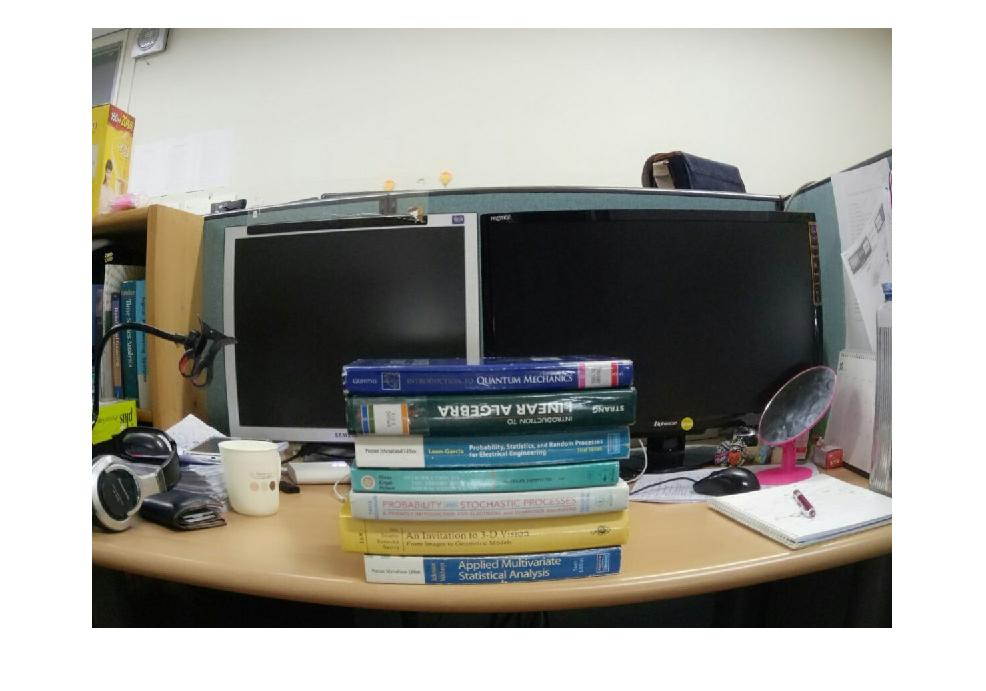
\includegraphics[scale=.3]{figures/assignment_02_figure_01.jpg}
        \caption{Original Image}
    \end{subfigure}\\
    \begin{subfigure}[h]{0.5\textwidth}
        \centering
        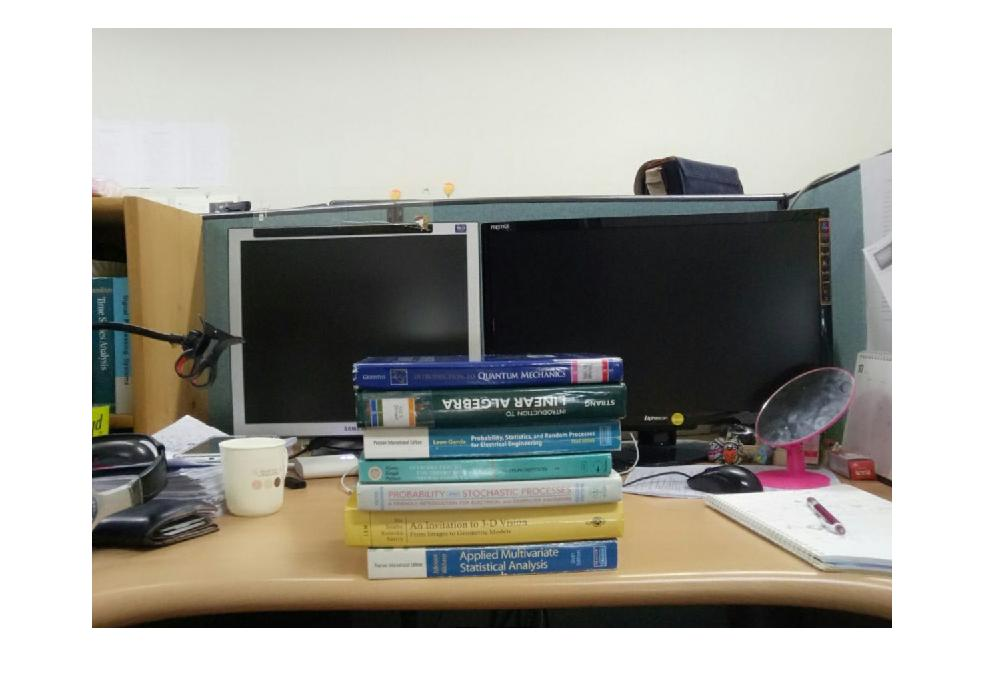
\includegraphics[scale=.3]{figures/assignment_02_figure_02.jpg}
        \caption{Unwraped Image}
    \end{subfigure}\\
\end{figure}

\end{homeworkProblem}

%----------------------------------------------------------------------------------------

\end{document}
